\documentclass[12pt,a4paper]{article}
\usepackage[utf8]{inputenc}
\usepackage[english,russian]{babel}
\usepackage[left=1cm,right=1cm,top=2cm,bottom=2cm,bindingoffset=0cm]{geometry} 
\usepackage{textcomp,latexsym,pb-diagram,amsopn} 
\usepackage{amsmath}
\usepackage{amsfonts}
\usepackage{amssymb}
\usepackage{makeidx}
\usepackage{amsmath}
\usepackage{amsfonts}
\usepackage{amssymb}
\usepackage{pdfpages}
\usepackage{cite,enumerate,float,indentfirst} 
\usepackage{graphicx,xcolor} 
\usepackage{float}
\usepackage{gnuplottex}
\usepackage{caption,setspace}
\captionsetup{font={small}}

\begin{document}
\title{Численное моделирование нестационарного течения газа с 
использованием разностной несимметричной схемы $Ln(p)$-СКОРОСТЬ}
\author{Бекбулатов Рамзан \\ 410 группа }

\maketitle

\section{\LARGE Тесты}

\subsection{ \Large Случай гладкого решения}
Проверка работоспособности схемы производилась для следующего гладкого решения:

\begin{figure}[h]
\center{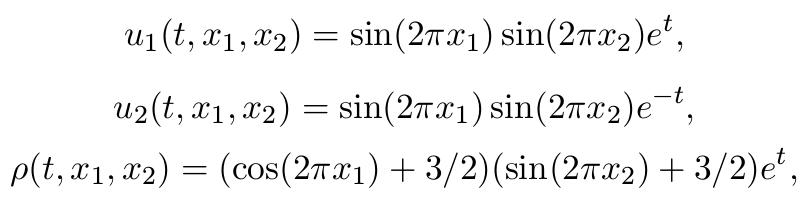
\includegraphics[width=0.5\linewidth]{./images/22.png}}
\end{figure}



\section{\LARGE Постановка задачи}
Решение краевой задачи протекания газа через область $\Omega$

Система уравнений, описывающая нестационарное движение баротропного газа в области $\Omega$ размерности 2 или 3, выглядит следующим образом

\begin{figure}[h]
\center{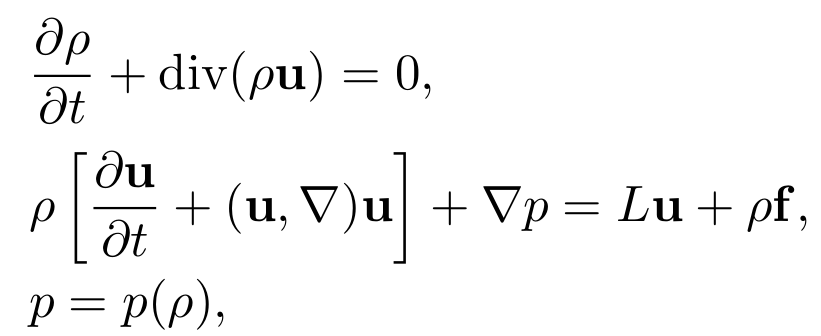
\includegraphics[width=0.4\linewidth]{./images/1.png}}
\end{figure}
где $L$ есть линейный симметричный положительно определенный оператор
\begin{figure}[h!]
\center{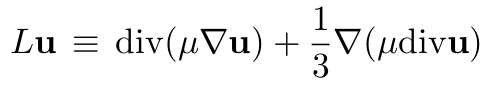
\includegraphics[width=0.35\linewidth]{./images/11.png}}
\end{figure}

Для построения разностной схемы в двумерном случае с односторонними разностями, направленными против потока, и вычисляемой функцией $g = ln(p)$ запишем систему в виде
\begin{figure}[h!]
\center{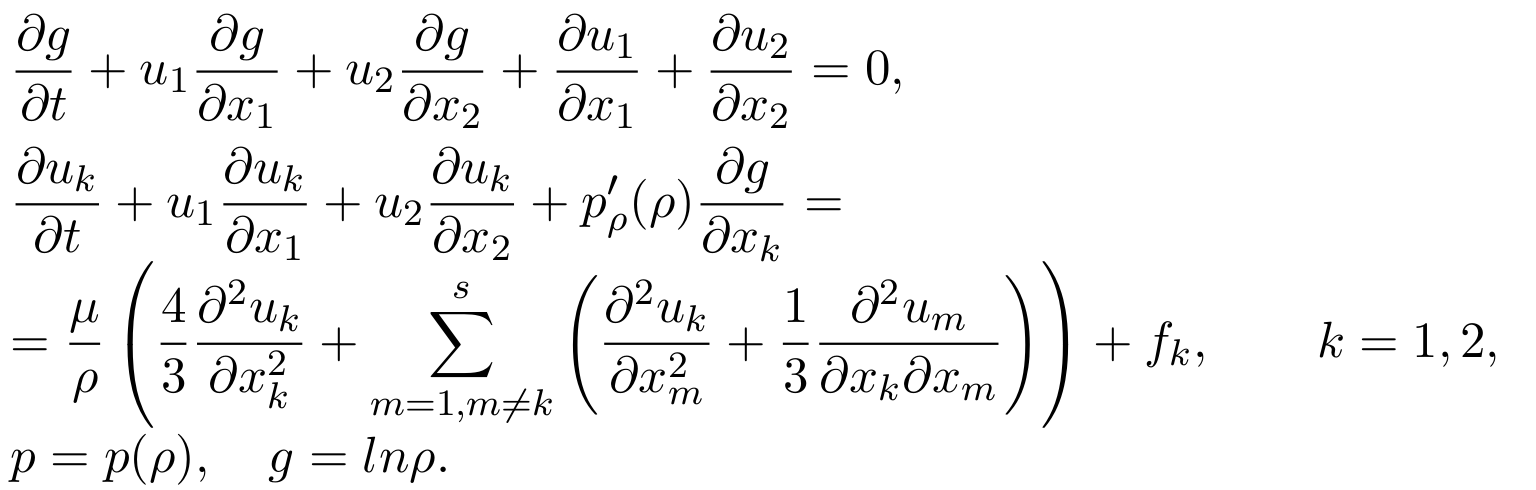
\includegraphics[width=0.8\linewidth]{./images/4.png}}
\end{figure}
\newpage
Неизвестные функции: плотность $p$ и вектор скорости $u$ являются функциями переменных Эйлера
\begin{figure}[h!] 
\center{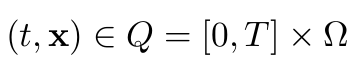
\includegraphics[width=0.27\linewidth]{./images/14.png}}
\end{figure}

В начальный момент времени задаются функции, значения которых определяют плотность и скорость газав каждой точке области $\Omega$:
\begin{figure}[h]
\center{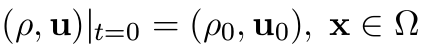
\includegraphics[width=0.3\linewidth]{./images/15.png}}
\end{figure}

\section{Область и граничные условия}
Компоненты функции скорости на границе области $\Omega$ будем считать равными нулю, если явно не задано другое условие. На границе, где вектор скорости направлен во внутрь, будем считать известной фукнцию плотности, положив её значение равным $\rho_{\gamma}$. На остальных участках границы функция плотности считается неизвестной и подлежит определению.

Обозначим через $\Omega_{nm}$ квадрат, координаты точек которого удовлетворяют неравенствам $n < x < n + 1$ и $m < y < m + 1$. Множества точек, составляюзие стороны квадрата $\Omega_{nm}$ обозначим $\Gamma^{x-}_{nm}$, $\Gamma^{x+}_{nm}$, $\Gamma^{y-}_{nm}$ и $\Gamma^{y+}_{nm}$, где индекс x или y означает, какая из координат на стороне является постоянной, а + или - означает максимальное или минимальное значение, которое принимает эта координата. С учетом этих обозначений область и начальные условия можно записать в следующем виде:
\begin{equation*}
\bar{\Omega} = \bar{\Omega}_{01}\cup\bar{\Omega}_{02}\cup\bar{\Omega}_{11}\cup\bar{\Omega}_{12}\cup\bar{\Omega}_{20}\cup\bar{\Omega}_{21}\cup\bar{\Omega}_{22};
\end{equation*}
\begin{equation*}
u_1(x, y) = w, \quad where \quad (x, y)\in \Gamma^{x-}_{01}\cup\Gamma^{x+}_{02};
\end{equation*}
\begin{equation*}
\dfrac{\partial u_2 (x, y)}{\partial y} = 0, \quad where \quad (x, y)\in \Gamma^{y-}_{20}
\end{equation*}



\section{\LARGE Алгоритм}

Используемые обозначения:
\begin{figure}[h!]
\center{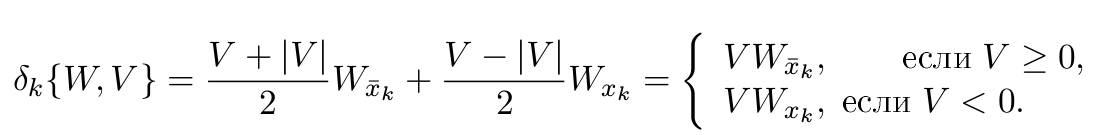
\includegraphics[width=0.6\linewidth]{./images/17.png}}
\center{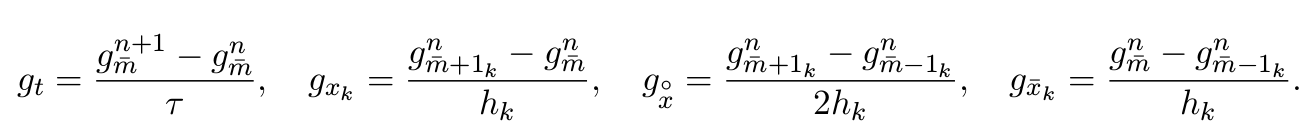
\includegraphics[width=0.8\linewidth]{./images/18.png}}
\end{figure} \\
Для поиска численного решения задачи предлагается использовать р.с.:
\begin{figure}[h!]
\center{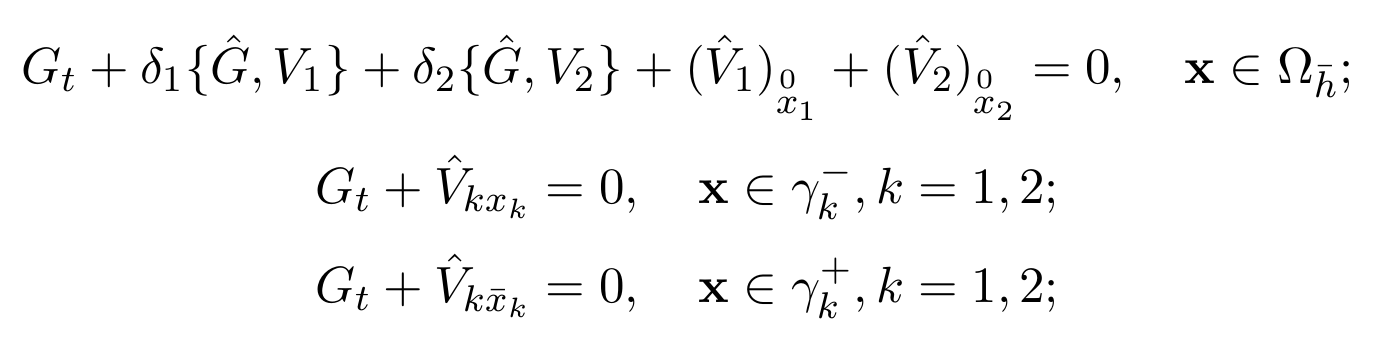
\includegraphics[width=0.6\linewidth]{./images/7.png}}
\center{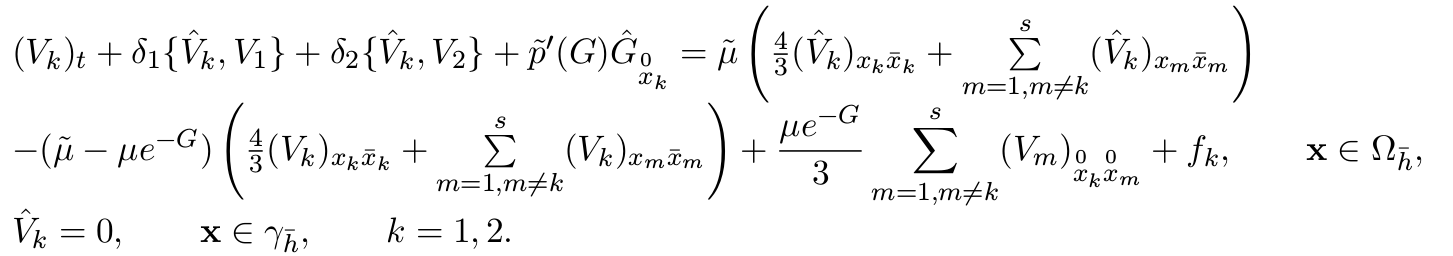
\includegraphics[width=0.9\linewidth]{./images/8.png}}
\end{figure} 
\begin{figure}[h!]
\center{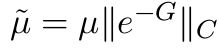
\includegraphics[width=0.16\linewidth]{./images/9.png}}
\end{figure} \\
\newpage
Приведем индексную запись уравнений данной разностной схемы:
\begin{figure}[h!]
\center{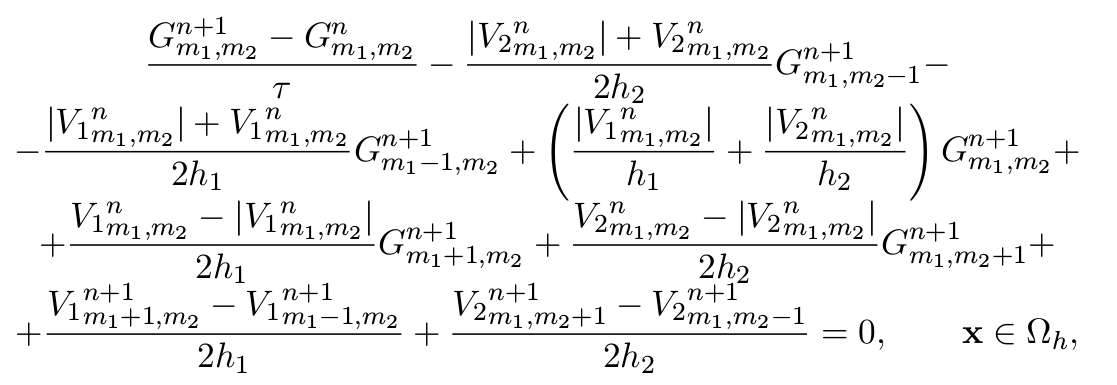
\includegraphics[width=0.75\linewidth]{./images/2.png}}
\end{figure}
\begin{figure}[h!]
\center{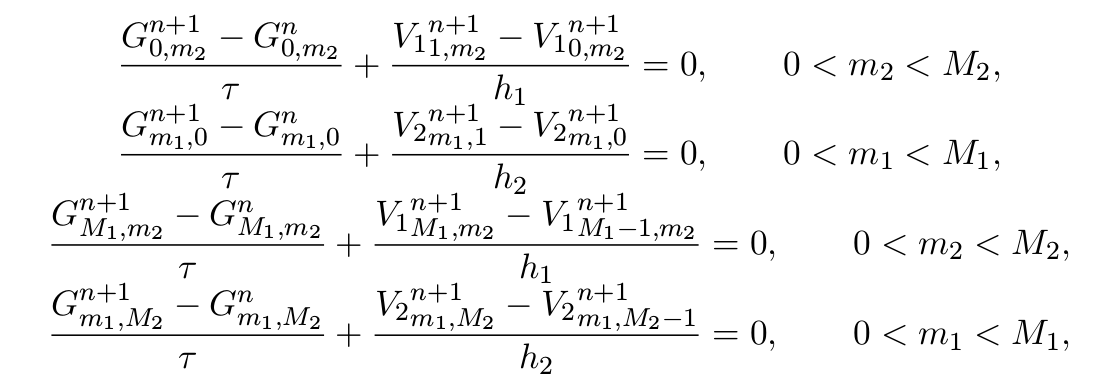
\includegraphics[width=0.75\linewidth]{./images/3.png}}
\end{figure}
\begin{figure}[h!]
\center{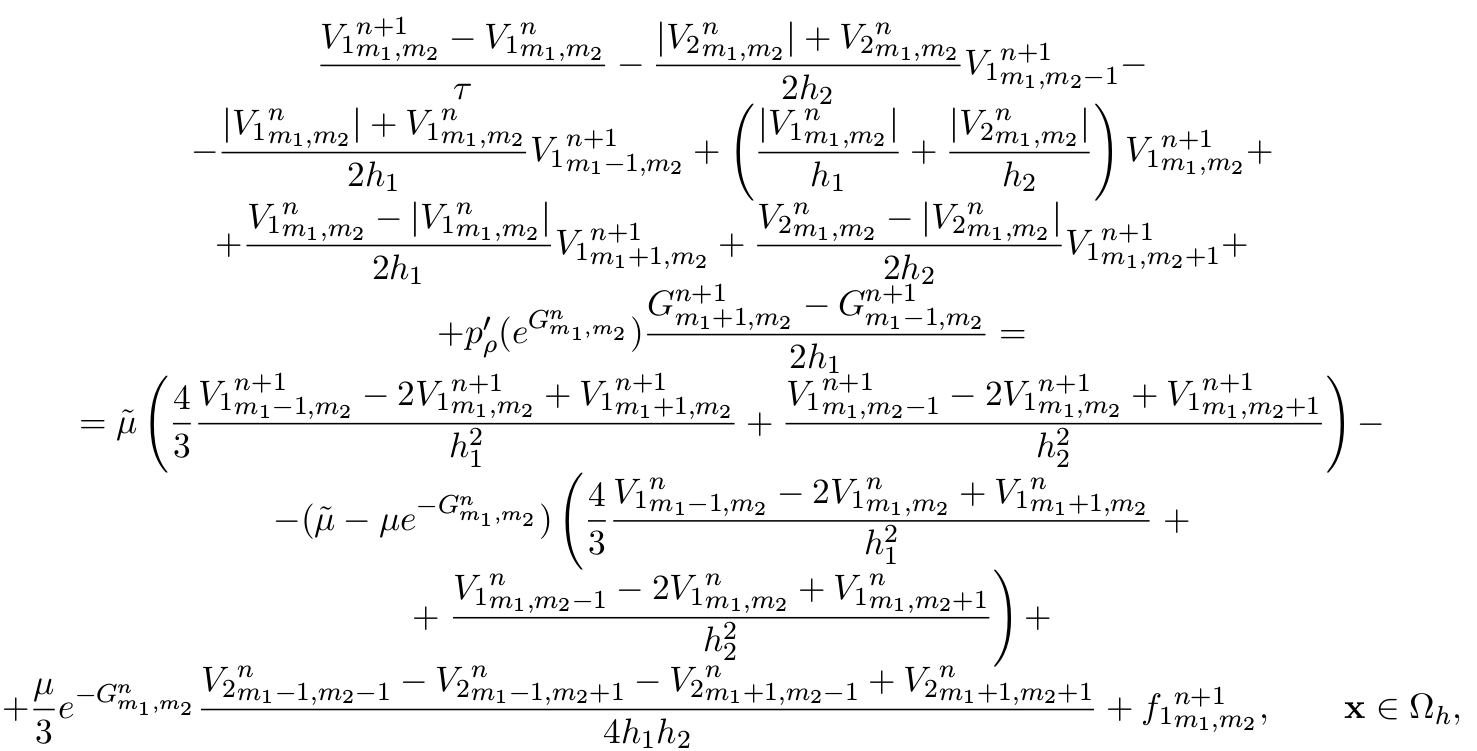
\includegraphics[width=0.95\linewidth]{./images/19.png}}
\end{figure}
\newpage
\begin{figure}[h!]
\center{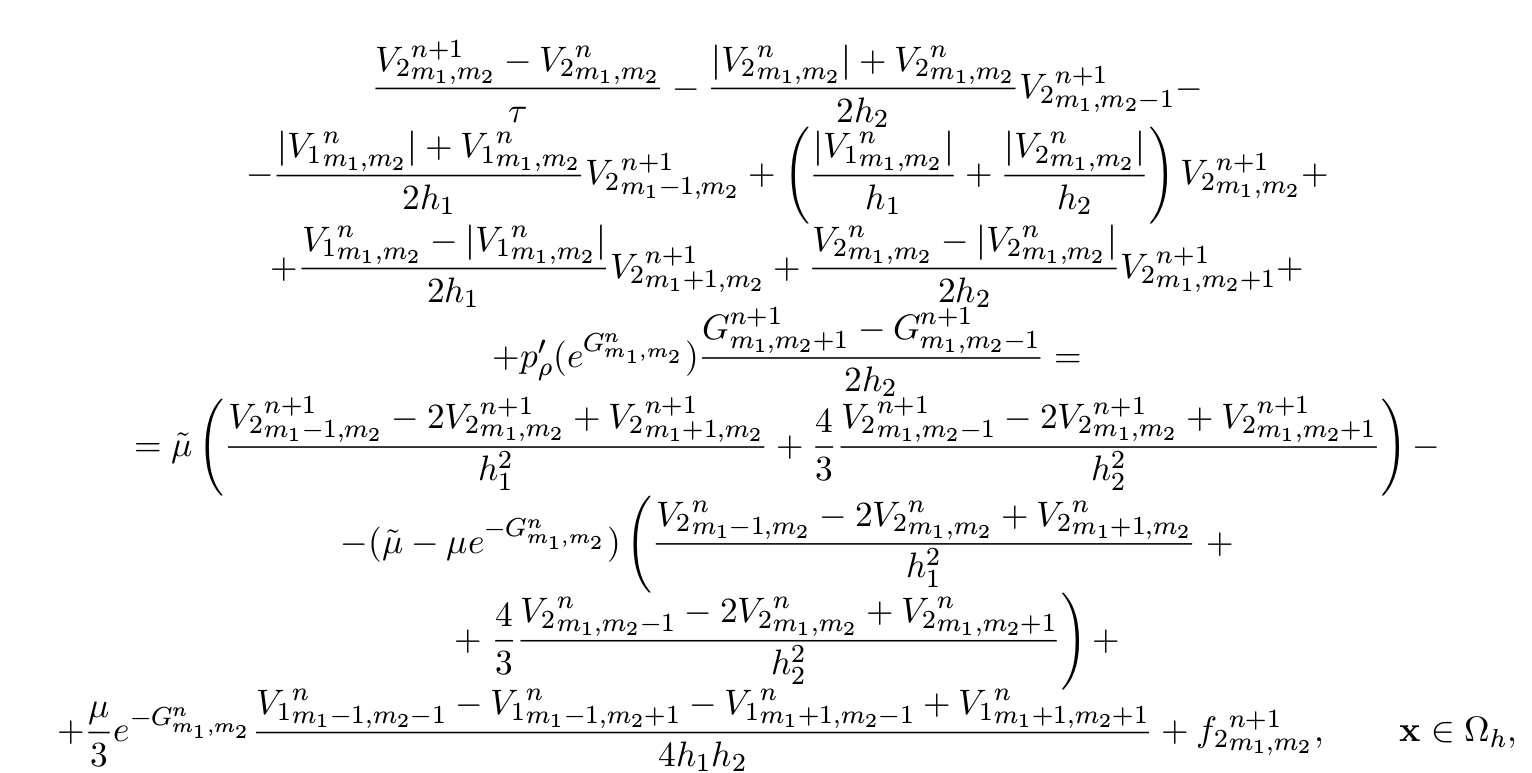
\includegraphics[width=0.95\linewidth]{./images/5.png}}
\end{figure} 
Данные уравнения образуют СЛАУ, решая которую находим сеточное решение на очередном слое.

Из первого разностного уравнения получаем следующие алгебраические уравнения для всех внутренних узлов:
\begin{figure}[h!]
{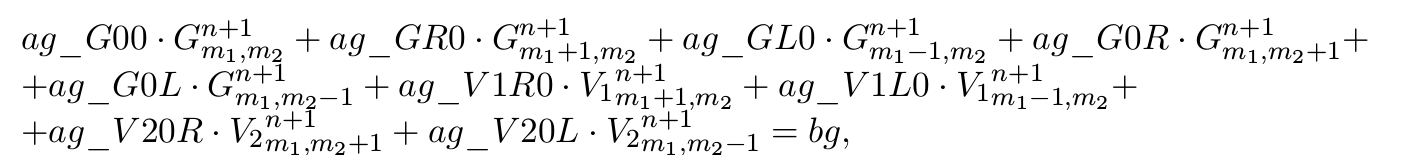
\includegraphics[width=0.93\linewidth]{./images/6.png}}
\end{figure} \\
где коэффициенты определяются по формулам:
\begin{figure}[h!]
{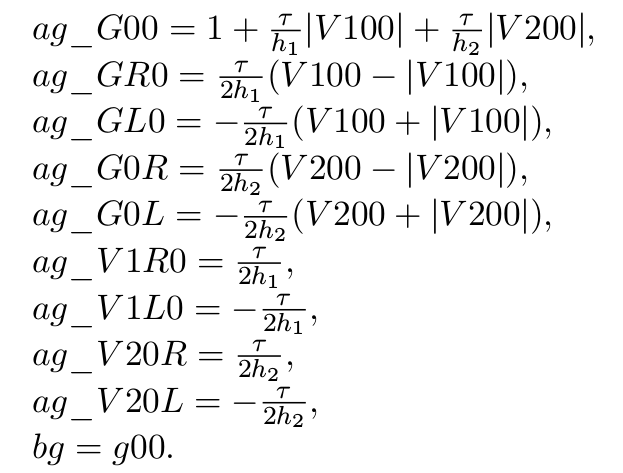
\includegraphics[width=0.38\linewidth]{./images/20.png}}
\end{figure} \\
Из третьего уравнения получаем: \\ \\
$ av1\_V100 \cdot (V_1)_{m_1,m_2}^{n+1} + av1\_V1R0 \cdot (V_1)_{m_1+1,m_2}^{n+1}
+ av1\_V1L0 \cdot (V_1)_{m_1-1,m_2}^{n+1} + av1\_V10R \cdot (V_1)_{m_1,m_2+1}^{n+1}
+ av1\_V10L \cdot (V_1)_{m_1,m_2-1}^{n+1} + av1\_GR0 \cdot G_{m_1 + 1,m_2}^{n+1}
+ av1\_GL0 * G_{m_1-1,m_2}^{n+1} = bv1,$ \\ \\
где \\ \\
$ av1\_V100 = 1 + \frac{\tau}{h_1}|V100| + \frac{\tau}{h_2}|V200| +  \tilde{\mu}\tau(\frac{8}{3h_1^2} + \frac{2}{h_2^2}) $ \\
$ av1\_V1L0 = -\frac{\tau}{2h_1}(|V100| + V100) - \frac{4\tilde \mu\tau}{3h_1^2} $ \\
$ av1\_V10L = -\frac{\tau}{2h_2}(|V200| + V200) - \frac{\tilde \mu\tau}  {h_2^2}  $ \\
$ av1\_V1R0 =  \frac{\tau}{2h_1}(V100 - |V100|) - \frac{4\tilde \mu\tau}{3h_1^2} $ \\
$ av1\_V10R =  \frac{\tau}{2h_2}(V200 - |V200|) - \frac{\tilde \mu\tau}  {h_2^2}  $ \\
$ av1\_GR0  =  \frac{\tau}{2h_1}\rho_p' $ \\
$ av1\_GL0  = -\frac{\tau}{2h_1}\rho_p' $
\begin{multline*}
bv1 = V100 + (-\tilde \mu + \mu e^{-g})(\frac{4\tau}{3h_1^2}(V1L0 - 2V1 + \\ +
  V1R0) + \frac{\tau}{h_2^2}(V10L - 2V1 + V10R)) +
  \\ + \frac{\mu\tau e^{-g}}{12h_1h_2}(V2LL - V2LR - V2RL + V2RR) + \tau F_{v2}
\end{multline*}
Из четвертого уравнения получаем: \\ \\
$ av2\_V200 \cdot (V_2)_{m_1,m_2}^{n+1} + av2\_V2R0 \cdot (V_2)_{m_1+1,m_2}^{n+1}
+ av2\_V2L0 \cdot (V_2)_{m_1-1,m_2}^{n+1} + av2\_V20R \cdot (V_2)_{m_1,m_2+1}^{n+1}
+ av2\_V20L \cdot (V_2)_{m_1,m_2-1}^{n+1} + av2\_GR0 \cdot G_{m_1 + 1,m_2}^{n+1}
+ av2\_GL0 * G_{m_1-1,m_2}^{n+1} = bv1,$ \\ \\
где \\ \\
$ av2\_V200 = 1 + \frac{\tau}{h_1}|V100| + \frac{\tau}{h_2}|V200| +  \tilde{\mu}\tau(\frac{8}{3h_2^2} + \frac{2}{h_1^2})$ \\
$ av2\_V2L0 = -\frac{\tau}{2h_1}(|V100| + V100) - \frac{\tilde \mu\tau}  {h_1^2}  $ \\
$ av2\_V20L = -\frac{\tau}{2h_2}(|V200| + V200) - \frac{4\tilde \mu\tau}{3h_2^2} $ \\
$ av2\_V2R0 =  \frac{\tau}{2h_1}(V100 - |V100|) - \frac{\tilde \mu\tau}  {h_1^2}  $ \\ 
$ av2\_V20R =  \frac{\tau}{2h_2}(V200 - |V200|) - \frac{4\tilde \mu\tau}{3h_2^2} $ \\
$ av2\_G0R  =  \frac{\tau}{2h_2}\rho_p'e^g $ \\
$ av2\_G0L  = -\frac{\tau}{2h_2}\rho_p'e^g $
\begin{multline*}
bv2 = V200 - (\tilde \mu - \mu e^{-g})(\frac{\tau}{h_1^2}(V2L0 - 2V2 +
\\ + V2R0) + \frac{4\tau}{3h_2^2}(V20L - 2V2 + V20R)) +
\\ + \frac{\mu\tau e^{-g}}{12h_1h_2}(V1LL - V1LR - V1RL + V1RR) + \tau F_{v2}
\end{multline*}

\section{Результаты расчета для гладкого решения}

Ниже представлена таблица точности расчетов для разных сеток. Из данных результатов следует, что точность вычислений 
возрастает при размельчении сетки.

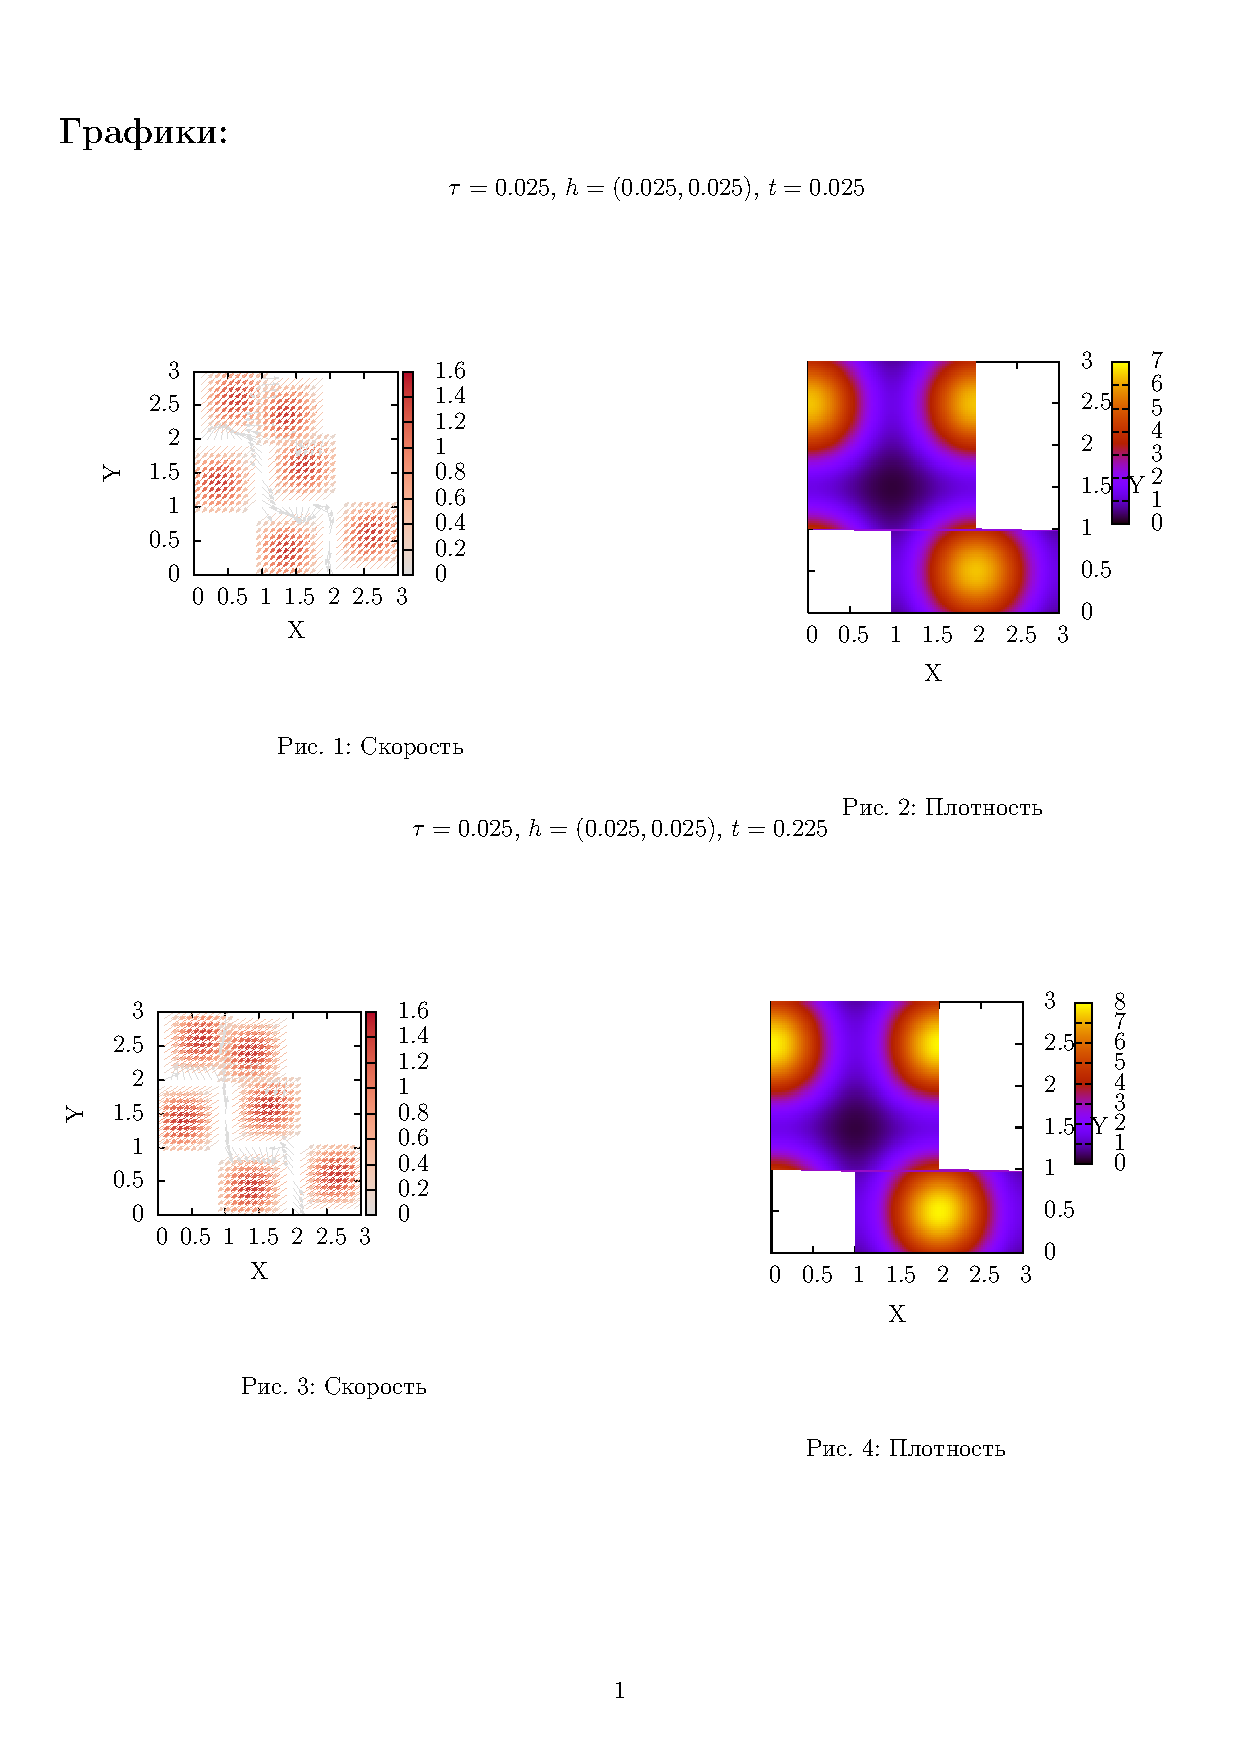
\includepdf[pages={-}]{plot_smooth.pdf}

 $norm\;of\;the\;error\;in\;C\;for\;g: \quad p_{\rho}=1.000, \mu = 0.100 \\ $
\begin{tabular}{|p{0.6in}|p{1.2in}|p{1.2in}|p{1.2in}|} \hline
$\tau\setminus h$ & $0.05000 $ & 0.02500 & 0.01250 \\ \hline
$0.05000$ & $9.908e-01$ &$6.824e-01$ &$5.356e-01$  \\ \hline
$0.02500$ & $8.234e-01$ &$4.873e-01$ &$3.289e-01$  \\ \hline
$0.01250$ & $7.447e-01$ &$4.048e-01$ &$2.403e-01$  \\ \hline
\end{tabular}\\[20pt]
  
$
 \text{norm of the error in $L_2$ for g}: \quad p_{\rho}=1.000, \mu = 0.100 \\ $
\begin{tabular}{|p{0.6in}|p{1.2in}|p{1.2in}|p{1.2in}|} \hline
$\tau\setminus h$ & $0.05000$ & $0.02500$& $0.01250$ \\ \hline
$0.05000$ & $1.840e-01$ &$1.263e-01$ &$1.007e-01$  \\ \hline
$0.02500$ & $1.482e-01$ &$8.847e-02$ &$6.119e-02$  \\ \hline
$0.01250$ & $1.321e-01$ &$7.177e-02$ &$4.345e-02$  \\ \hline
\end{tabular}\\[20pt]
 

 $norm\;of\;the\;error\;in\;C\;for\;v1: \quad p_{\rho}=1.000, \mu = 0.100 $ \\ 
\begin{tabular}{|p{0.6in}|p{1.2in}|p{1.2in}|p{1.2in}|} \hline
$\tau\setminus h$ & $0.05000 $ & 0.02500 & 0.01250 \\ \hline
$0.05000$ & $4.664e-01$ &$3.455e-01$ &$2.847e-01$  \\ \hline
$0.02500$ & $4.361e-01$ &$2.800e-01$ &$1.969e-01$  \\ \hline
$0.01250$ & $4.255e-01$ &$2.570e-01$ &$1.558e-01$  \\ \hline
\end{tabular}\\[20pt]
  

 $norm\;of\;the\;error\;in\;L_2\;for\;v1: \quad p_{\rho}=1.000, \mu = 0.100 $ \\ 
\begin{tabular}{|p{0.6in}|p{1.2in}|p{1.2in}|p{1.2in}|} \hline
$\tau\setminus h$ & $0.05000 $ & 0.02500 & 0.01250 \\ \hline
$0.05000$ & $1.374e-01$ &$9.638e-02$ &$7.556e-02$  \\ \hline
$0.02500$ & $1.275e-01$ &$7.925e-02$ &$5.293e-02$  \\ \hline
$0.01250$ & $1.247e-01$ &$7.271e-02$ &$4.298e-02$  \\ \hline
\end{tabular}\\[20pt]
 
\newpage

 $norm\;of\;the\;error\;in\;C\;for\;v2: \quad p_{\rho}=1.000, \mu = 0.100 $ \\ 
\begin{tabular}{|p{0.6in}|p{1.2in}|p{1.2in}|p{1.2in}|} \hline
$\tau\setminus h$ & $0.05000 $ & 0.02500 & 0.01250 \\ \hline
$0.05000$ & $2.871e-01$ &$1.967e-01$ &$1.564e-01$  \\ \hline
$0.02500$ & $2.492e-01$ &$1.519e-01$ &$1.022e-01$  \\ \hline
$0.01250$ & $2.277e-01$ &$1.297e-01$ &$7.782e-02$  \\ \hline
\end{tabular}\\[20pt]
  

 $norm\;of\;the\;error\;in\;L_2\;for\;v2: \quad p_{\rho}=1.000, \mu = 0.100 $ \\ 
\begin{tabular}{|p{0.6in}|p{1.2in}|p{1.2in}|p{1.2in}|} \hline
$\tau\setminus h$ & $0.05000 $ & 0.02500 & 0.01250 \\ \hline
$0.05000$ & $9.131e-02$ &$6.581e-02$ &$5.306e-02$  \\ \hline
$0.02500$ & $7.585e-02$ &$4.852e-02$ &$3.433e-02$  \\ \hline
$0.01250$ & $6.821e-02$ &$4.009e-02$ &$2.508e-02$  \\ \hline
\end{tabular}\\[20pt]
 

 $ time, p_{\rho}=1.000, \mu = 0.100 $ \\ 
\begin{tabular}{|p{0.6in}|p{1.2in}|p{1.2in}|p{1.2in}|} \hline
$\tau\setminus h$ & $0.05000 $ & 0.02500 & 0.01250 \\ \hline
$0.05000$ & $7.056e-01$ &$4.954e+00$ &$4.219e+01$  \\ \hline
$0.02500$ & $1.091e+00$ &$6.653e+00$ &$4.727e+01$  \\ \hline
$0.01250$ & $1.772e+00$ &$1.036e+01$ &$6.161e+01$  \\ \hline
\end{tabular}\\[20pt]
 


\section{Результаты расчета задачи протекания}
После отладки схемы на гладком решении были проведен расчет задачи протекания при различных значения параметров $\rho_{\gamma}$ и $w$. Ниже представлены результаты.

\subsection{Графики при $\rho_{0} = 0.5, \rho_{\gamma} = 0.3, w = 0.1$}
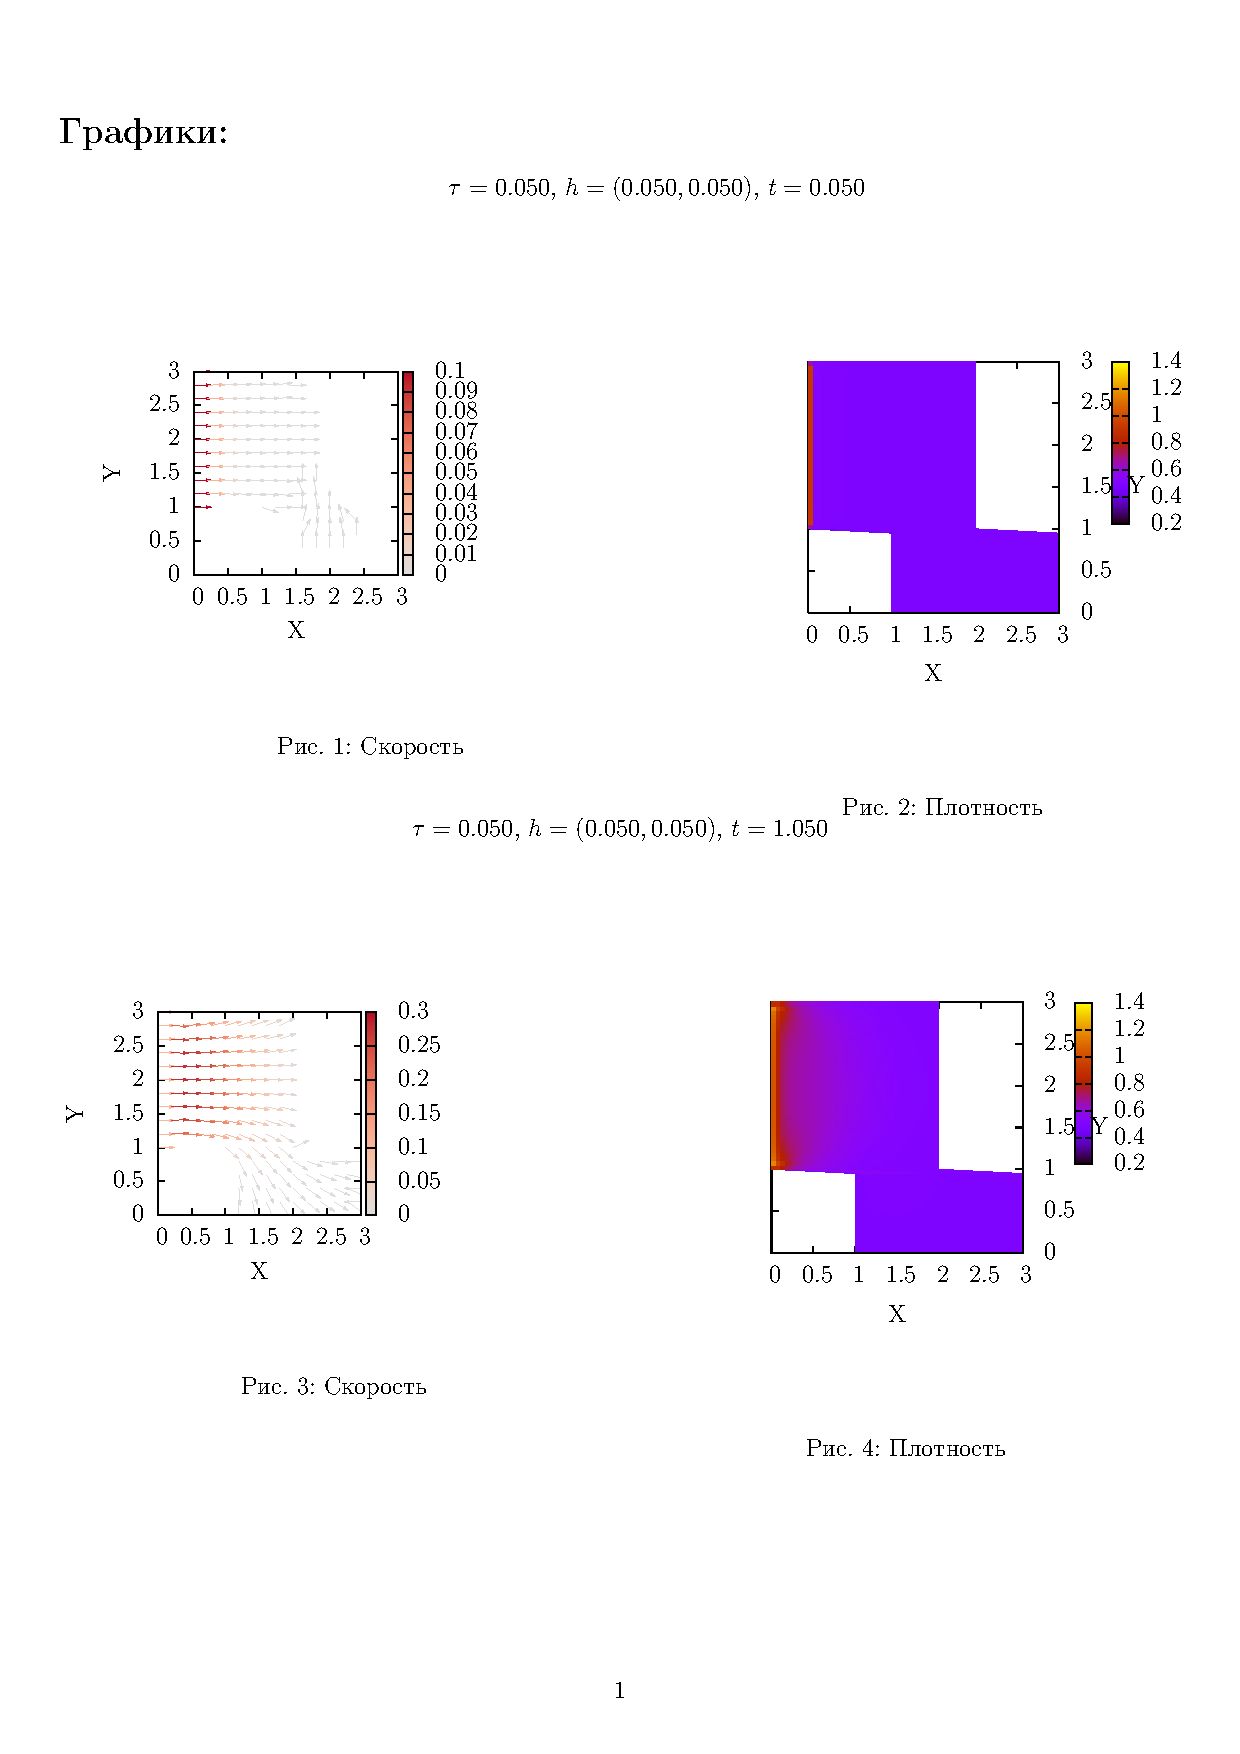
\includepdf[pages={-}]{plot_abrupt_5_3_1.pdf}

\subsection{Графики при $\rho_{0} = 0.5, \rho_{\gamma} = 0.3, w = 0.5$}
Эти графики отображают моделирование более быстрого втекания газа. \\
Видны небольшие ударные волны.
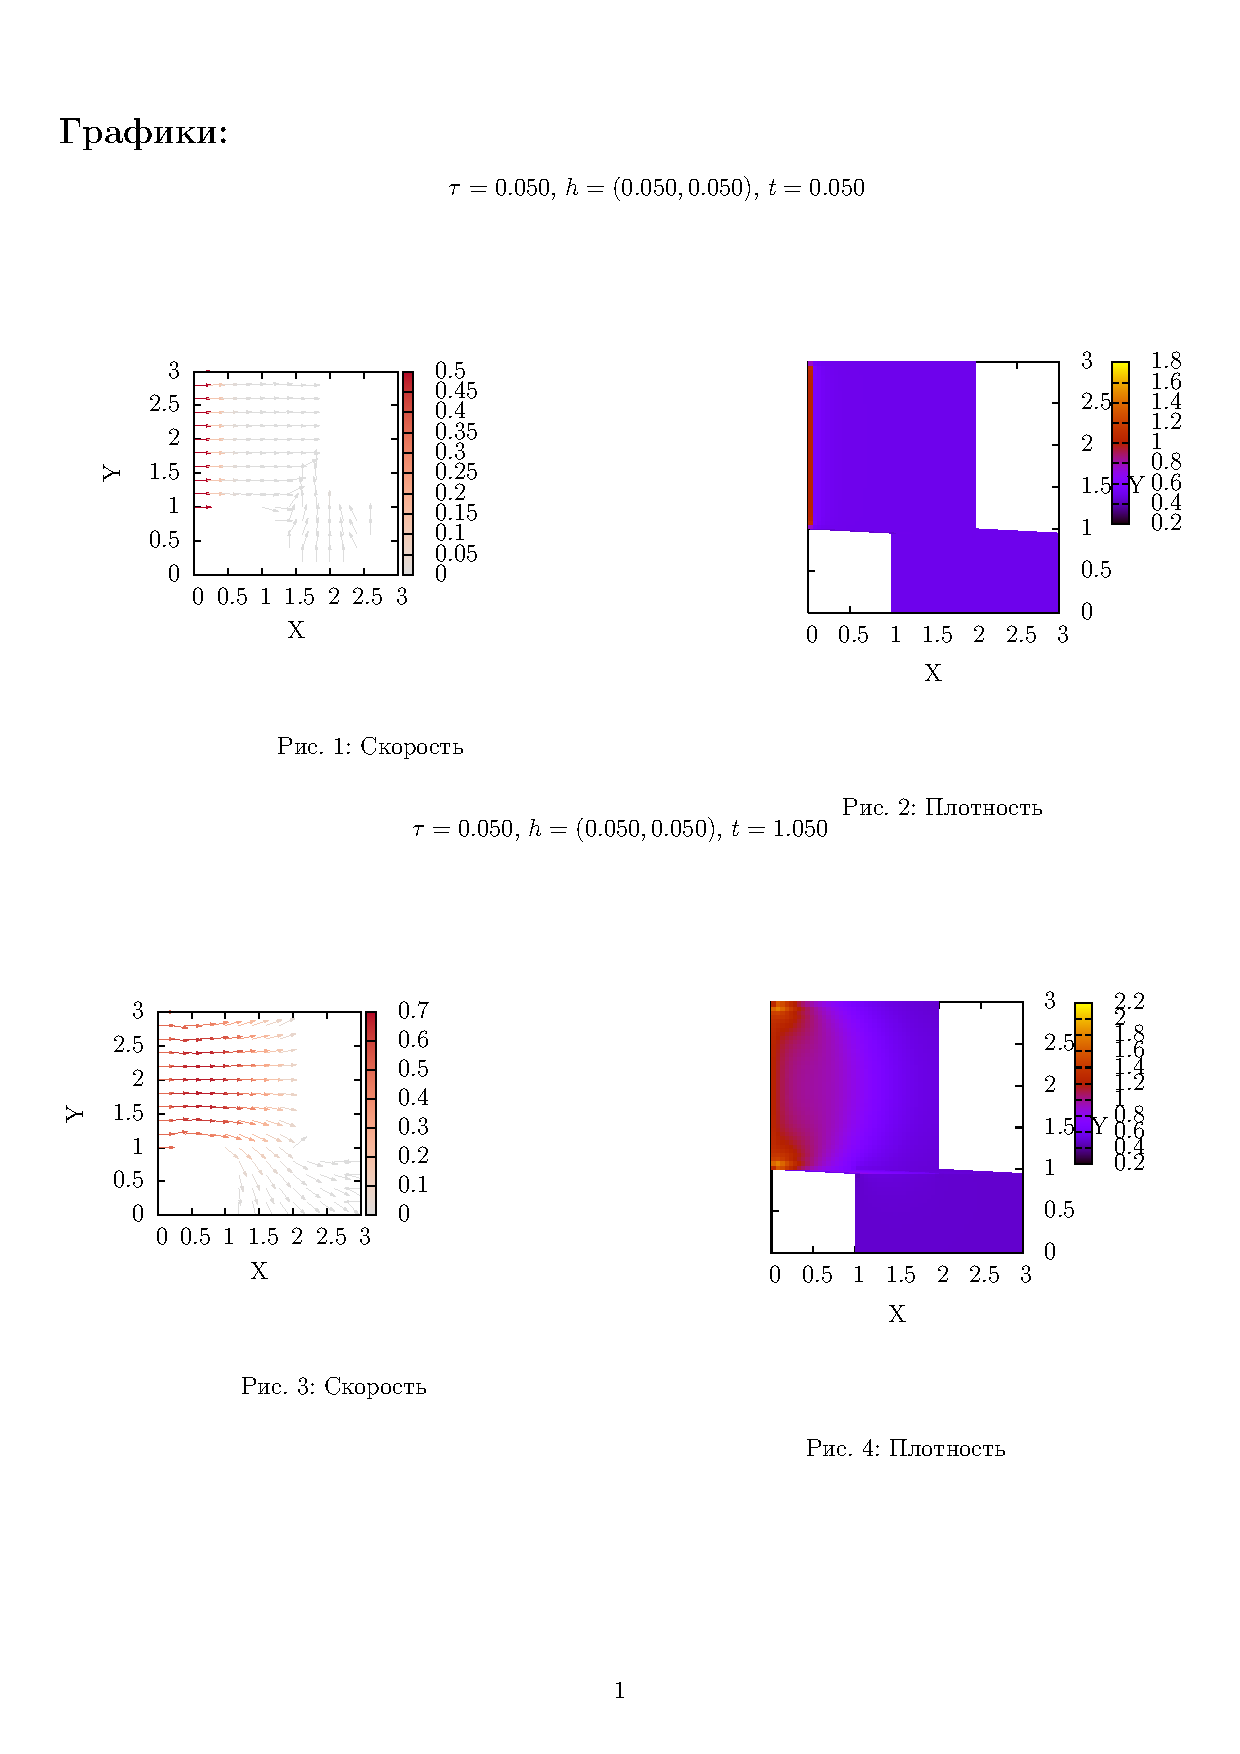
\includepdf[pages={-}]{plot_abrupt_5_3_5.pdf}

\subsection{Графики при $\rho_{0} = 0.5, \rho_{\gamma} = 0.3, w = 1.0$}
Эти графики отображают моделирование еще более быстрого втекания газа. \\
Видны сильные ударные волны и завихрения.
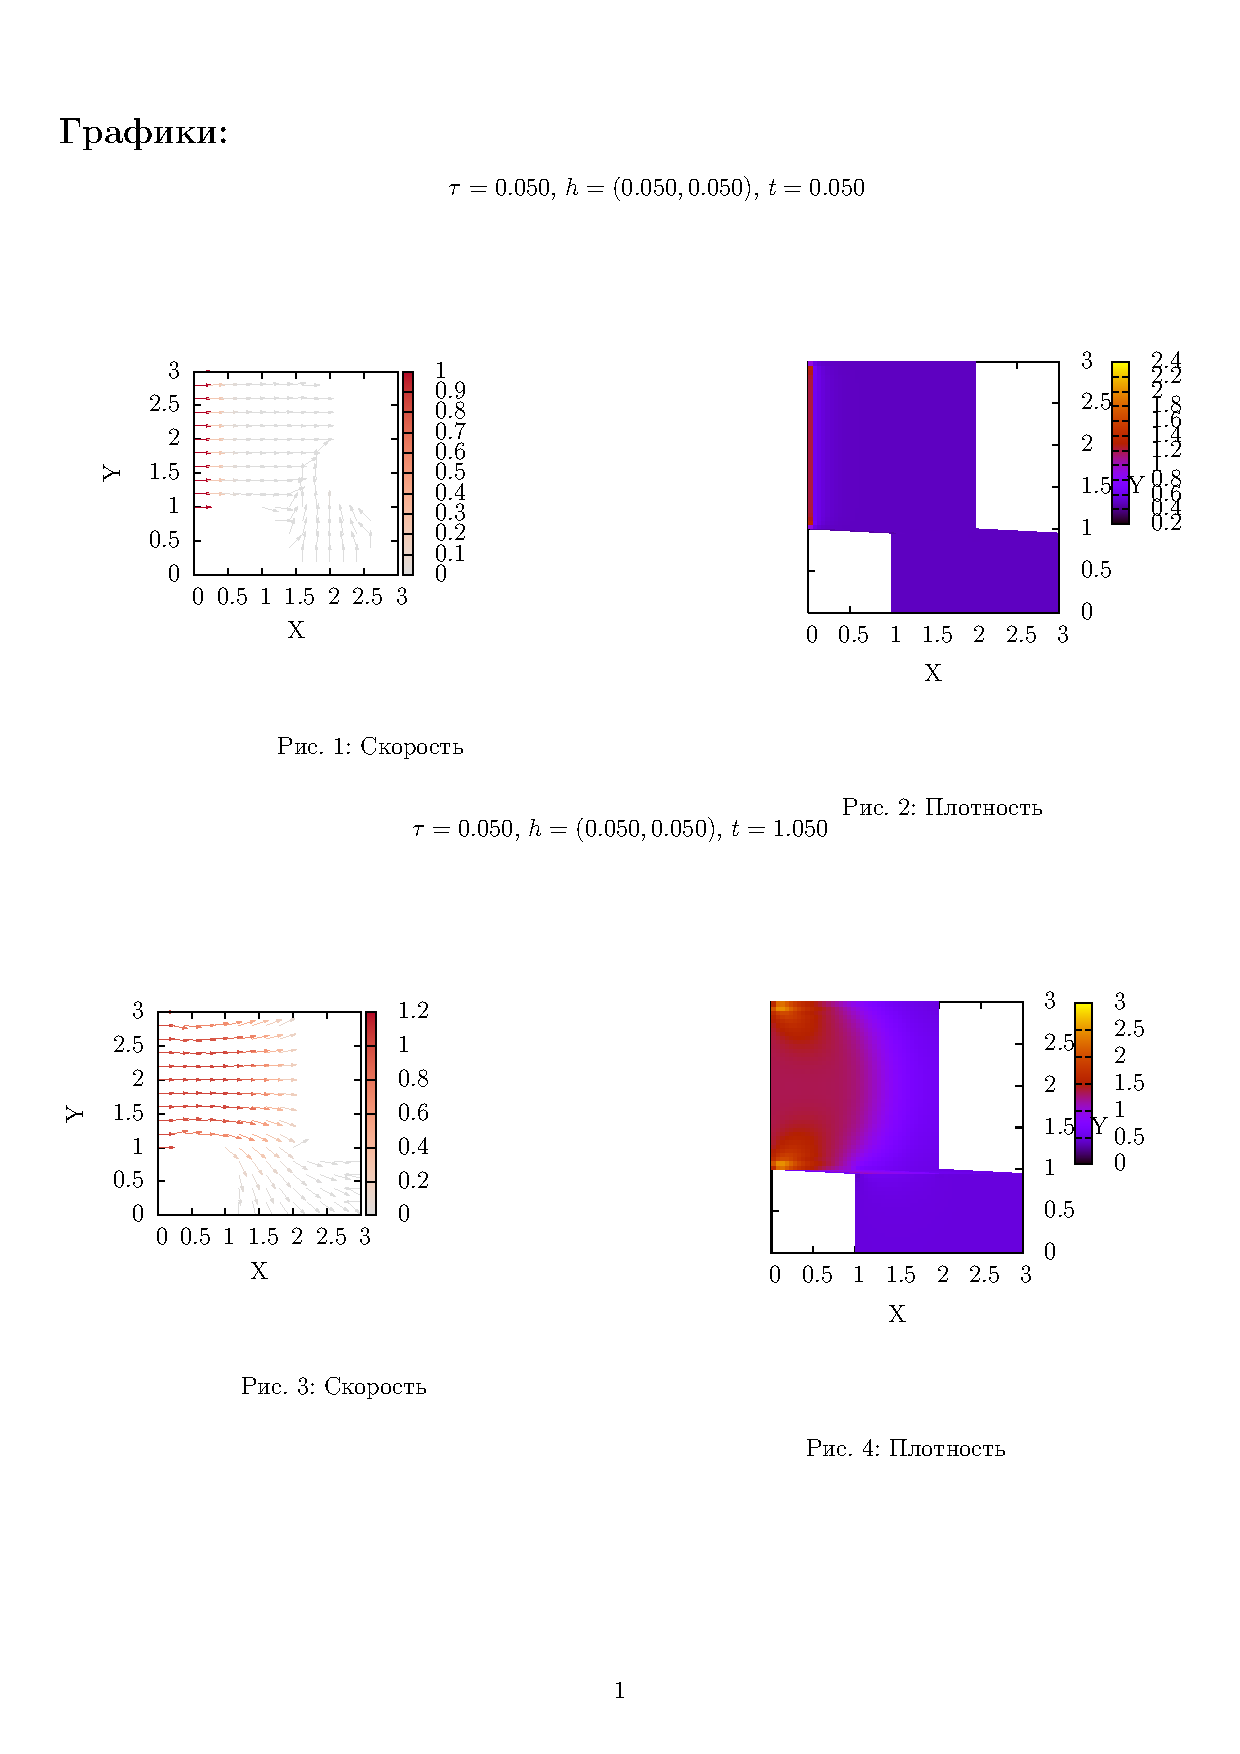
\includepdf[pages={-}]{plot_abrupt_5_3_10.pdf}

\subsection{Графики при $\rho_{0} = 0.1, \rho_{\gamma} = 0.5, w = 0.1$}
Эти графики отображают моделирование медленного втекания плотного газа в разреженную среду.
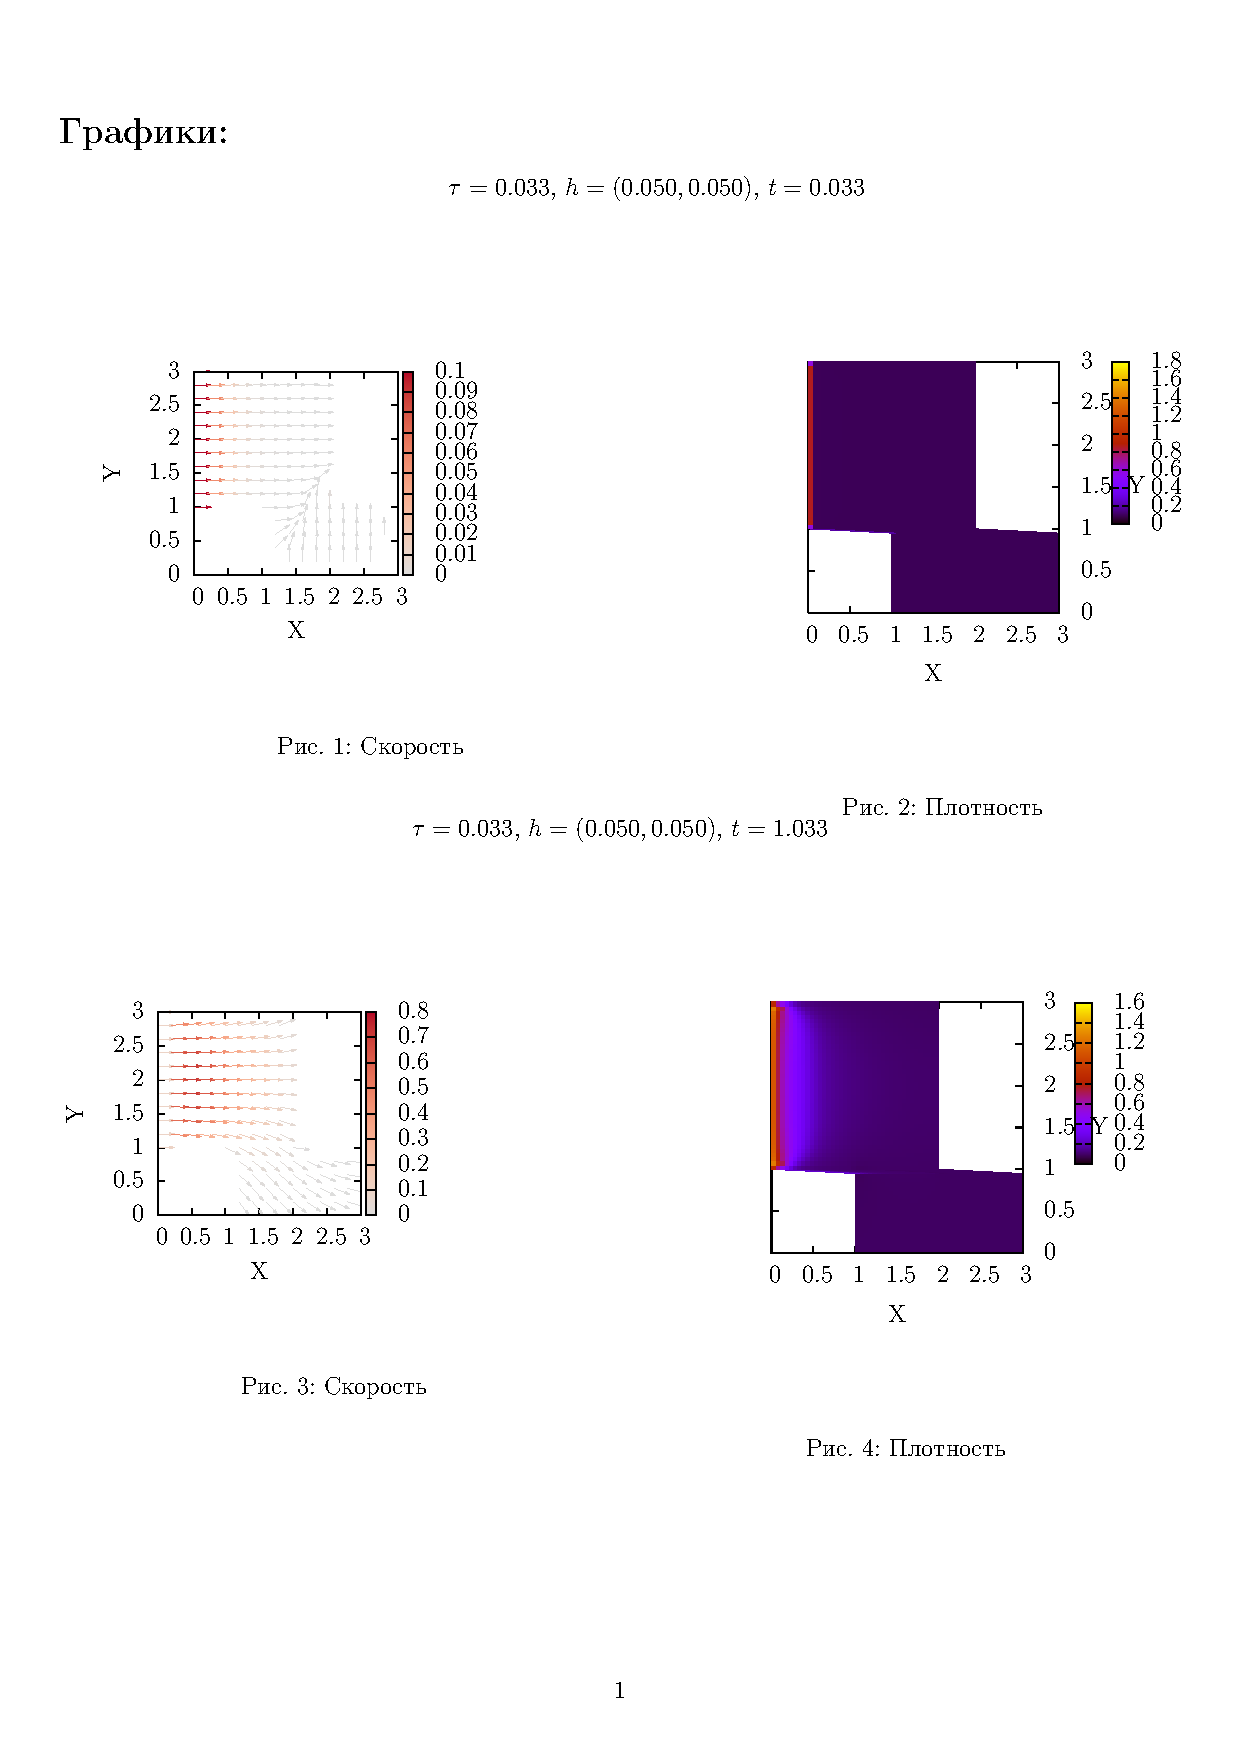
\includepdf[pages={-}]{plot_abrupt_1_5_1.pdf}

\section{Спектр линеризованного разностного оператора}
Стационарное решение было найдено следующим способом: на итерациях проверялась норма текущего решения по сравнению с предыдущим. Критерием выхода было выбрано значение $eps = 1.e-12$. Стационарное решение было найдено:
\begin{center}
N = 4000, M1 =  60, M2 =  60, Dim =   2521.                 \\
t =    1, norm = 1.072538e-01                               \\
t =  100, norm = 1.942510e-03                               \\
t =  200, norm = 9.581218e-04                               \\
t =  300, norm = 5.200315e-04                               \\
t =  400, norm = 2.968678e-04                               \\
t =  500, norm = 1.745928e-04                               \\
t =  600, norm = 1.046111e-04                               \\
t =  700, norm = 6.341809e-05                               \\
t =  800, norm = 3.872874e-05                               \\
t =  900, norm = 2.375964e-05                               \\
t = 1000, norm = 1.461777e-05                               \\
t = 1100, norm = 9.009206e-06                               \\
t = 1200, norm = 5.558587e-06                               \\
t = 1300, norm = 3.431910e-06                               \\
t = 1400, norm = 2.119779e-06                               \\
t = 1500, norm = 1.309666e-06                               \\
t = 1600, norm = 8.092901e-07                               \\
t = 1700, norm = 5.001458e-07                               \\
t = 1800, norm = 3.091189e-07                               \\
t = 1900, norm = 1.910678e-07                               \\
t = 2000, norm = 1.181082e-07                               \\
t = 2100, norm = 7.301506e-08                               \\
t = 2200, norm = 4.513974e-08                               \\
t = 2300, norm = 2.790872e-08                               \\
t = 2400, norm = 1.725944e-08                               \\
t = 2500, norm = 1.067561e-08                               \\
t = 2600, norm = 6.602656e-09                               \\
t = 2700, norm = 4.090830e-09                               \\
t = 2800, norm = 2.530869e-09                               \\
t = 2900, norm = 1.569131e-09                               \\
t = 3000, norm = 9.622032e-10                               \\
t = 3100, norm = 5.999068e-10                               \\
t = 3200, norm = 3.692501e-10                               \\
t = 3300, norm = 1.493756e-10                               \\
t = 3400, norm = 6.684053e-11                               \\
Stationary solution has been found at T = 3485.             \\
Current norm = 0.000000e+00, criteria norm = 1.000000e-12.  \\
Elapsed time: 30.28 sec.                                    \\
\end{center}
 
Рассмотрим линеризацию разностного оператора на стационарном решении:
\begin{figure}[h!]
\center{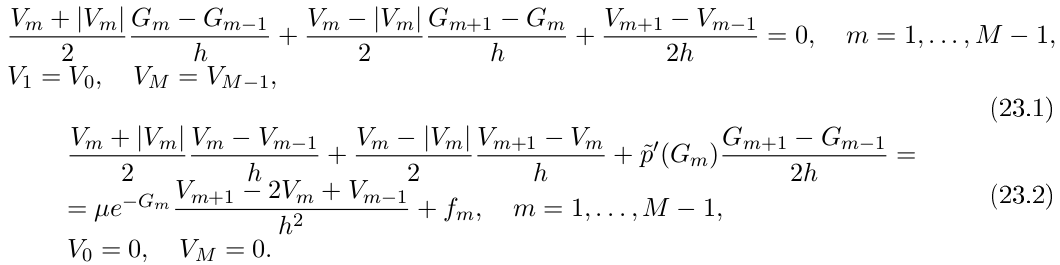
\includegraphics[width=0.8\linewidth]{./images/linear231.png}}
\end{figure}
\begin{figure}[h!]
\center{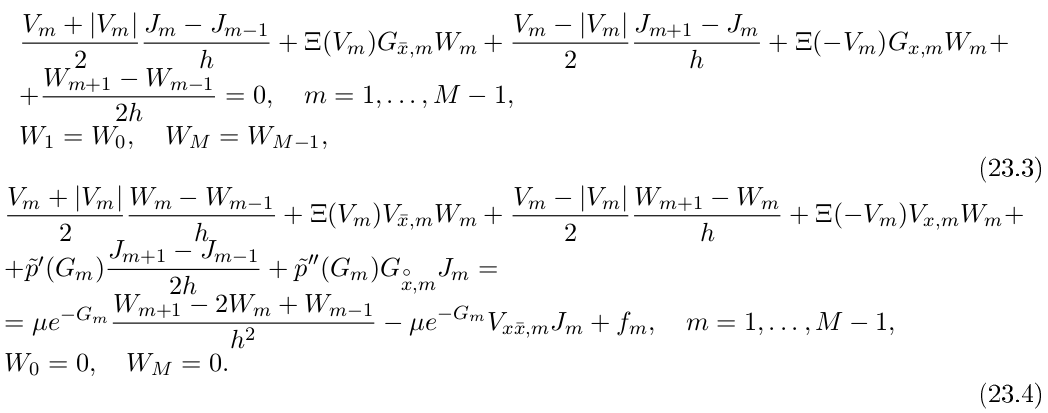
\includegraphics[width=0.8\linewidth]{./images/linear232.png}}
\end{figure}
\begin{figure}[h!]
\center{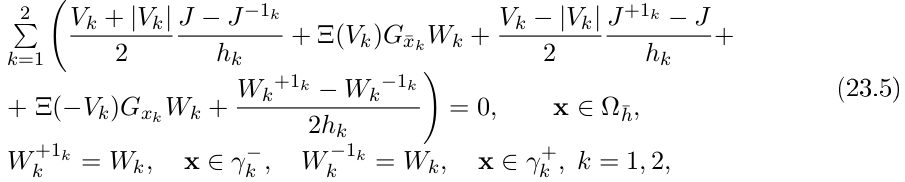
\includegraphics[width=0.8\linewidth]{./images/linear233.png}}
\end{figure}
\begin{figure}[h!]
\center{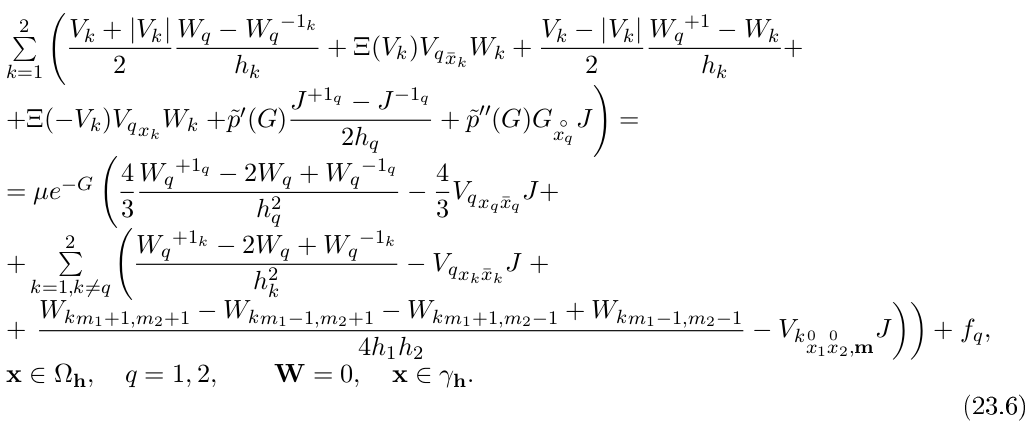
\includegraphics[width=0.8\linewidth]{./images/linear234.png}}
\end{figure}
\newpage

С помощью метода Арнольди было найдены собственные значения задачи. Приведем 6 значений с  максимальным модулем действительной части:
\begin{eqnarray*}
	Accuracy = 1.00e-12 \\
	\lambda_1 = 3.45916e+02 + 0.00000e+00 * i, |\lambda_1| = 3.45916e+02 \\
	\lambda_2 = 3.43587e+02 + 0.00000e+00 * i, |\lambda_2| = 3.43587e+02 \\ 
	\lambda_3 = 3.43352e+02 + 0.00000e+00 * i, |\lambda_3| = 3.43352e+02 \\
	\lambda_4 = 3.41391e+02 + 0.00000e+00 * i, |\lambda_4| = 3.41391e+02 \\
	\lambda_5 = 3.35196e+02 + 0.00000e+00 * i, |\lambda_5| = 3.35196e+02 \\
	\lambda_6 = 3.35173e+02 + 0.00000e+00 * i, |\lambda_6| = 3.35173e+02
\end{eqnarray*}

Далее собственная функция, соответствующая $\lambda_1$, была добавлена к стационарному решению исходной задачи протекания для проверки стабилизации.

После применения первой собственной функции решение стабилизировалось:
\begin{center}
N = 4000, M1 =  60, M2 =  60, Dim =   2921. \\
t =   1, norm = 9.215979e-03 \\
t =  50, norm = 1.518452e-06 \\
t = 100, norm = 3.177534e-07 \\
t = 150, norm = 7.196107e-08 \\
t = 200, norm = 1.957946e-08 \\
t = 250, norm = 6.958395e-09 \\
t = 300, norm = 3.082941e-09 \\
t = 350, norm = 1.640359e-09 \\
t = 400, norm = 7.533327e-10 \\
t = 450, norm = 4.580188e-10 \\
t = 500, norm = 3.245409e-10 \\
t = 550, norm = 1.305495e-10 \\
t = 600, norm = 1.155570e-10 \\
t = 650, norm = 6.031444e-11 \\
t = 700, norm = 5.705633e-11 \\
t = 750, norm = 5.282850e-11 \\
Solution has stabilized at T = 765. \\
Accuracy = 1.000000e-12. \\
Elapsed time: 2.99 sec.
\end{center}

Для второй собственной функции решение также стабилизировалось:
\begin{center}
N = 4000, M1 =  60, M2 =  60, Dim =   2921. \\
t =   1, norm = 1.011079e-02 \\
t =  50, norm = 1.417708e-06 \\
t = 100, norm = 4.218732e-07 \\
t = 150, norm = 2.141778e-07 \\
t = 200, norm = 1.073394e-07 \\
t = 250, norm = 6.270735e-08 \\
t = 300, norm = 4.627349e-08 \\
t = 350, norm = 3.026252e-08 \\
t = 400, norm = 2.535985e-08 \\
t = 450, norm = 1.995482e-08 \\
t = 500, norm = 1.575544e-08 \\
t = 550, norm = 1.284315e-08 \\
t = 600, norm = 1.021578e-08 \\
t = 650, norm = 8.217876e-09 \\
t = 700, norm = 6.610261e-09 \\
t = 750, norm = 5.300305e-09 \\
t = 800, norm = 4.264015e-09 \\
t = 850, norm = 3.424477e-09 \\
t = 900, norm = 2.740526e-09 \\
t = 950, norm = 2.204339e-09 \\
t = 1000, norm = 1.772738e-09 \\
t = 1050, norm = 1.425979e-09 \\
t = 1100, norm = 1.147007e-09 \\
t = 1150, norm = 9.225735e-10 \\
t = 1200, norm = 7.154950e-10 \\
t = 1250, norm = 5.940779e-10 \\
t = 1300, norm = 4.452441e-10 \\
t = 1350, norm = 3.760065e-10 \\
t = 1400, norm = 2.590215e-10 \\
t = 1450, norm = 1.568099e-10 \\
t = 1500, norm = 1.335894e-10 \\
t = 1550, norm = 1.159368e-10 \\
t = 1600, norm = 5.868843e-11 \\
t = 1650, norm = 5.481610e-11 \\
Solution has stabilized at T = 1700. \\
Accuracy = 1.000000e-12. \\
Elapsed time: 6.50 sec.
\end{center}

Для третьей собственной функции решение также стабилизировалось:
\begin{center}
N = 4000, M1 =  60, M2 =  60, Dim =   2921. \\
t =   1, norm = 9.912132e-03 \\
t =  50, norm = 1.449576e-06 \\
t = 100, norm = 3.966946e-07 \\
t = 150, norm = 1.852152e-07 \\
t = 200, norm = 9.138744e-08 \\
t = 250, norm = 5.380196e-08 \\
t = 300, norm = 3.989353e-08 \\
t = 350, norm = 2.634723e-08 \\
t = 400, norm = 2.208830e-08 \\
t = 450, norm = 1.737300e-08 \\
t = 500, norm = 1.373932e-08 \\
t = 550, norm = 1.119461e-08 \\
t = 600, norm = 8.905537e-09 \\
t = 650, norm = 7.165152e-09 \\
t = 700, norm = 5.763338e-09 \\
t = 750, norm = 4.621504e-09 \\
t = 800, norm = 3.717908e-09 \\
t = 850, norm = 2.972228e-09 \\
t = 900, norm = 2.386171e-09 \\
t = 950, norm = 1.919893e-09 \\
t = 1000, norm = 1.543961e-09 \\
t = 1050, norm = 1.242012e-09 \\
t = 1100, norm = 9.990294e-10 \\
t = 1150, norm = 8.035519e-10 \\
t = 1200, norm = 6.463658e-10 \\
t = 1250, norm = 5.175611e-10 \\
t = 1300, norm = 3.917659e-10 \\
t = 1350, norm = 2.996897e-10 \\
t = 1400, norm = 2.493009e-10 \\
t = 1450, norm = 1.878360e-10 \\
t = 1500, norm = 1.556930e-10 \\
t = 1550, norm = 6.017516e-11 \\
t = 1600, norm = 5.600955e-11 \\
t = 1650, norm = 5.231857e-11 \\
Solution has stabilized at T = 1666. \\
Accuracy = 1.000000e-12. \\
Elapsed time: 6.34 sec.
\end{center}


Для четвертой собственной функции решение также стабилизировалось:
\begin{center}
N = 4000, M1 =  60, M2 =  60, Dim =   2921. \\
t =   1, norm = 1.014023e-02 \\
t =  50, norm = 1.520263e-06 \\
t = 100, norm = 4.294082e-07 \\
t = 150, norm = 2.072974e-07 \\
t = 200, norm = 9.915863e-08 \\
t = 250, norm = 5.018681e-08 \\
t = 300, norm = 3.102233e-08 \\
t = 350, norm = 1.662699e-08 \\
t = 400, norm = 1.369804e-08 \\
t = 450, norm = 1.040108e-08 \\
t = 500, norm = 8.050092e-09 \\
t = 550, norm = 6.651140e-09 \\
t = 600, norm = 5.224934e-09 \\
t = 650, norm = 4.220633e-09 \\
t = 700, norm = 3.398249e-09 \\
t = 750, norm = 2.702803e-09 \\
t = 800, norm = 2.179913e-09 \\
t = 850, norm = 1.751594e-09 \\
t = 900, norm = 1.408692e-09 \\
t = 950, norm = 1.133770e-09 \\
t = 1000, norm = 9.115799e-10 \\
t = 1050, norm = 7.333935e-10 \\
t = 1100, norm = 5.765073e-10 \\
t = 1150, norm = 4.620610e-10 \\
t = 1200, norm = 3.438024e-10 \\
t = 1250, norm = 2.623456e-10 \\
t = 1300, norm = 1.406415e-10 \\
t = 1350, norm = 1.719932e-10 \\
t = 1400, norm = 1.476308e-10 \\
t = 1450, norm = 5.828311e-11 \\
t = 1500, norm = 5.445164e-11 \\
Solution has stabilized at T = 1546. \\
Accuracy = 1.000000e-12. \\
Elapsed time: 5.87 sec.
\end{center}

Для пятой собственной функции решение также стабилизировалось:
\begin{center}
N = 4000, M1 =  60, M2 =  60, Dim =   2921. \\
t =   1, norm = 9.142406e-03 \\
t =  50, norm = 2.048954e-06 \\
t = 100, norm = 4.258540e-07 \\
t = 150, norm = 9.387426e-08 \\
t = 200, norm = 2.342738e-08 \\
t = 250, norm = 7.580249e-09 \\
t = 300, norm = 3.920671e-09 \\
t = 350, norm = 3.003094e-09 \\
t = 400, norm = 2.045663e-09 \\
t = 450, norm = 1.701500e-09 \\
t = 500, norm = 1.353527e-09 \\
t = 550, norm = 1.064288e-09 \\
t = 600, norm = 8.708926e-10 \\
t = 650, norm = 6.725304e-10 \\
t = 700, norm = 5.532713e-10 \\
t = 750, norm = 4.075822e-10 \\
t = 800, norm = 3.572455e-10 \\
t = 850, norm = 2.921970e-10 \\
t = 900, norm = 2.284302e-10 \\
t = 950, norm = 1.642103e-10 \\
t = 1000, norm = 6.579885e-11 \\
t = 1050, norm = 5.768013e-11 \\
t = 1100, norm = 5.386698e-11 \\
Solution has stabilized at T = 1132. \\
Accuracy = 1.000000e-12. \\
Elapsed time: 3.84 sec.
\end{center}

Для шестой собственной функции решение также стабилизировалось:
\begin{center}
N = 4000, M1 =  60, M2 =  60, Dim =   2921. \\
t =   1, norm = 9.921207e-03 \\
t =  50, norm = 1.579346e-06 \\
t = 100, norm = 4.347833e-07 \\
t = 150, norm = 2.039629e-07 \\
t = 200, norm = 9.631162e-08 \\
t = 250, norm = 4.664720e-08 \\
t = 300, norm = 2.623964e-08 \\
t = 350, norm = 1.270969e-08 \\
t = 400, norm = 1.000848e-08 \\
t = 450, norm = 7.254256e-09 \\
t = 500, norm = 5.529269e-09 \\
t = 550, norm = 4.608453e-09 \\
t = 600, norm = 3.575317e-09 \\
t = 650, norm = 2.890150e-09 \\
t = 700, norm = 2.325523e-09 \\
t = 750, norm = 1.858544e-09 \\
t = 800, norm = 1.501712e-09 \\
t = 850, norm = 1.205667e-09 \\
t = 900, norm = 9.696615e-10 \\
t = 950, norm = 7.805736e-10 \\
t = 1000, norm = 6.241177e-10 \\
t = 1050, norm = 4.746564e-10 \\
t = 1100, norm = 3.655697e-10 \\
t = 1150, norm = 2.774617e-10 \\
t = 1200, norm = 2.449538e-10 \\
t = 1250, norm = 1.389234e-10 \\
t = 1300, norm = 1.204065e-10 \\
t = 1350, norm = 5.985902e-11 \\
t = 1400, norm = 5.583457e-11 \\
t = 1450, norm = 5.215090e-11 \\
Solution has stabilized at T = 1463. \\
Accuracy = 1.000000e-12. \\
Elapsed time: 5.58 sec.
\end{center}

Рассмотренные собственные значения отличаются по модулю в пределах 2\%, однако времена стабилизации (T) решения при соответствующих возмущениях могут отличаться существенно.

\end{document}


